%!TEX TS-program = xelatex
%!TEX encoding = UTF-8 Unicode
%!TEX root = 2020-GS-ARTICLE.tex
%----------------------------------------------------------------- LANGUAGES ---
\newcommand{\mylanguages}{english,italian} % in reverse order
%---------------------------------------------------------- TITLE & SUBTITLE ---
\newcommand{\mytitle}{Stereophonic Mathematical Models}
\newcommand{\mysubtitle}{Stereophonic Mathematical Models}
%----------------------------------------------------------------- AUTHOR(s) ---
\newcommand{\authorone}{Perla Catucci}
\newcommand{\institutione}{Conservatorio N. Piccinni di Bari}
\newcommand{\emailone}{perlacatucci150 @ gmail.com}
%-------------------------------------------------------------------------------
\newcommand{\authortwo}{Michele Ruzzi}
\newcommand{\institutiontwo}{Conservatorio N. Piccinni di Bari}
\newcommand{\emailtwo}{m.ruzzi @ icloud.com} % duplicate these 3 lines if more
%-------------------------------------------------------------------------------
\newcommand{\authorthree}{Giuseppe Silvi}
\newcommand{\institutionthree}{Conservatorio N. Piccinni di Bari}
\newcommand{\emailthree}{grammaton @ me.com} % duplicate these 3 lines if more
%-------------------------------------------------------------- STYLE GS2020 ---
%!TEX TS-program = xelatex
%!TEX encoding = UTF-8 Unicode
%!TEX root = 2020-GS-ARTICLE.tex
%-------------------------------- PACKAGES AND OTHER DOCUMENT CONFIGURATIONS ---
\documentclass[
	a4paper,
	twocolumn
]{article}
\usepackage[
	top=20mm,
	bottom=25mm,
	textwidth=17.2cm,
	columnsep=0.8cm
]{geometry}
\usepackage[T1]{fontenc}
\usepackage[\mylanguages]{babel}
\usepackage{graphicx}
\usepackage{dblfloatfix}
\usepackage{graphicx}
\usepackage{epstopdf}
\epstopdfsetup{update}
\usepackage[usenames]{color}
\usepackage{xcolor}
\usepackage{amssymb}
\usepackage{hyperref} % For hyperlinks in the PDF
\usepackage{Alegreya}
\linespread{1.05}
\usepackage{
	fontspec,
	xltxtra,
	xunicode
	}
\usepackage{
	xfrac,
	unicode-math
	}

\defaultfontfeatures{Mapping=tex-text}
\setmonofont[
	Scale=MatchLowercase
	]{Andale Mono}
\setmathfont[
	Scale=MatchLowercase,
	Scale=1
	]{Libertinus Math}

\usepackage{microtype}

\usepackage[
	hang,
	small,
	labelfont=bf,
	up,
	textfont=it,
	up
	]{caption}
\usepackage{paralist} % For compact item lists
\usepackage{etoolbox} % Some tools: used for quote environment
\AtBeginEnvironment{quote}{\small}
\usepackage{titling} % Customizing the title section
\usepackage{booktabs} % Horizontal rules in tables
\usepackage{enumitem} % Customized lists
\setlist[itemize]{noitemsep} % Make itemize lists more compact
\usepackage{abstract} % Allows abstract customization
\renewcommand{\abstractnamefont}{\normalfont\bfseries} % Set the "Abstract" text to bold
\renewcommand{\abstracttextfont}{\normalfont\small\itshape} % Set the abstract itself to small italic text
\usepackage{titlesec} % Allows customization of titles
\renewcommand\thesection{\Roman{section}} % Roman numerals for the sections
\renewcommand\thesubsection{\Roman{subsection}} % roman numerals for subsections
\titleformat{\section}[block]{\Large}{\thesection.}{1em}{} % Change the look of the section titles
\titleformat{\subsection}[block]{\large}{\thesubsection.}{1em}{} % Change the look of the section titles
%------------------------------------------------------------- TITLE SECTION ---
\setlength{\droptitle}{-4\baselineskip} % Move the title up
\pretitle{\begin{center}\huge\bfseries} % Article title formatting
\posttitle{\end{center}} % Article title closing formatting
\title{\mytitle \\[0.1cm] \large{\emph{\mysubtitle}}} % Article title
\author{%
\textsc{\authorone}\\%
\normalsize \institutione \\ %
\normalsize \emailone \\%
% activate
\and % duplicate these 4 lines if more
\textsc{\authortwo} \\%
\normalsize \institutiontwo \\ %
\normalsize \emailtwo \\%
\and % duplicate these 4 lines if more
\textsc{\authorthree} \\%
\normalsize \institutionthree \\ %
\normalsize \emailthree %
}
\date{} % Leave empty to omit a date

\usepackage{fancyhdr} % Headers and footers
\pagestyle{fancy} % All pages have headers and footers
\fancyhead{} % Blank out the default header
\fancyfoot{} % Blank out the default footer
\fancyhead[C]{\small Stereophonic Mathematical Models} % Custom header text
\fancyfoot[RO,LE]{\small \today~ • w: \input{includes/words.txt} • c: \input{includes/char.txt} • p:~\thepage} % Custom footer text
%-------------------------------------------------------------------------------
%-------------------------------------------------------------------------------
%	LISTINGS
%-------------------------------------------------------------------------------
%-------------------------------------------------------------------------------
\usepackage{listings}
% lstlistings setup
\definecolor{gsbg}{rgb}{0.98,0.98,0.98}

\lstset{%
  aboveskip=10pt,
	belowskip=5pt,
  language=C++,
  numbers=none,%left,%none,
  tabsize=4,
  %frame=single,
  breaklines=true,
  numberstyle=\tiny\ttfamily,
  backgroundcolor=\color{gsbg},
  basicstyle=\footnotesize\ttfamily,
  %commentstyle=\slshape\color{mylstcmt}, %\itshape,
  %frameround=tttt,
  columns=flexible, %fixed,
  showstringspaces=false,
  emptylines=2,
  inputencoding=utf8,
  extendedchars=true,
  literate=	{á}{{\'a}}1
			{à}{{\`a}}1
			{ä}{{\"a}}1
			{â}{{\^a}}1
			{é}{{\'e}}1
			{è}{{\`e}}1
			{ë}{{\"e}}1
			{ê}{{\^e}}1
			{ï}{{\"i}}1
			{î}{{\^i}}1
			{ö}{{\"o}}1
			{ô}{{\^o}}1
			{è}{{\`e}}1
			{ù}{{\`u}}1
			{û}{{\^u}}1
			{ç}{{\c{c}}}1
			{Ç}{{\c{C}}}1,
  emph={component, declare, environment, import, library, process},
  emph={[2]ffunction, fconstant, fvariable},
  emph={[3]button, checkbox, vslider, hslider, nentry, vgroup, hgroup, tgroup, vbargraph, hbargraph, attach},
  %emphstyle=\color{yotxt}, %\underline, %\bfseries,
  %morecomment=[s][\color{mylstdoc}]{<mdoc>}{</mdoc>},
  rulecolor=\color{black}
}

\usepackage[framemethod=tikz]{mdframed} % Allows defining custom boxed/framed environments

%-------------------------------------------------------------------------------
%--------------------------------------------------- INFORMATION ENVIRONMENT ---
%-------------------------------------------------------------------------------

% Usage:
% \begin{info}[optional title, defaults to "Info:"]
% 	contents
% 	\end{info}

\mdfdefinestyle{info}{%
	topline=false, bottomline=false,
	leftline=false, rightline=false,
	nobreak,
	singleextra={%
		\fill[black](P-|O)circle[radius=0.4em];
		\node at(P-|O){\color{white}\scriptsize\bf i};
		\draw[very thick](P-|O)++(0,-0.8em)--(O);%--(O-|P);
	}
}

% Define a custom environment for information
\newenvironment{info}[1][Info:]{ % Set the default title to "Info:"
	\medskip
	\begin{mdframed}[style=info]
		\noindent{\textbf{#1}}
}{
	\end{mdframed}
}

%-------------------------------------------------------------------------------
%----------------------------------------------------- BIOGRAFIA ENVIRONMENT ---
%-------------------------------------------------------------------------------

% Usage:
% \begin{bio}[optional title, defaults to "Info:"]
% 	contents
% 	\end{bio}

\mdfdefinestyle{bio}{%
	topline=false, bottomline=false,
	leftline=false, rightline=false,
	nobreak,
	singleextra={%
		\fill[black](P-|O)circle[radius=0.4em];
		\node at(P-|O){\color{white}\scriptsize\bf b};
		\draw[very thick](P-|O)++(0,-0.8em)--(O);%--(O-|P);
	}
}

% Define a custom environment for information
\newenvironment{bio}[1][Biografia:]{ % Set the default title to "Info:"
	\medskip
	\begin{mdframed}[style=bio]
		\noindent{\textbf{#1}}
}{
	\end{mdframed}
}

%-------------------------------------------------------------------------------
%------------------------------------------------------- WARNING ENVIRONMENT ---
%-------------------------------------------------------------------------------

% Usage:
% \begin{warn}[optional title, defaults to "Warning:"]
%	Contents
% \end{warn}

\mdfdefinestyle{warning}{
	topline=false, bottomline=false,
	leftline=false, rightline=false,
	nobreak,
	singleextra={%
		\draw(P-|O)++(-0.5em,0)node(tmp1){};
		\draw(P-|O)++(0.5em,0)node(tmp2){};
		\fill[black,rotate around={45:(P-|O)}](tmp1)rectangle(tmp2);
		\node at(P-|O){\color{white}\scriptsize\bf !};
		\draw[very thick](P-|O)++(0,-1em)--(O);%--(O-|P);
	}
}

% Define a custom environment for warning text
\newenvironment{warn}[1][Warning:]{ % Set the default warning to "Warning:"
	\medskip
	\begin{mdframed}[style=warning]
		\noindent{\textbf{#1}}
}{
	\end{mdframed}
}

%-------------------------------------------------------------------- ABSTRACT -
\renewcommand{\maketitlehookd}{%
\begin{abstract}
\noindent\input{includes/abstract.txt}
\end{abstract}
}

%------------------------------------------------------------ BEGIN DOCUMENT ---
\begin{document}
\maketitle
\thispagestyle{empty}
%-------------------------------------------------------------------- ABSTRACT -
% The abstract is an external txt file inside the includes folder
%-------------------------------------------------------------------------------
%-------------------------------------------------------------------------------
%---------------------------------------------------------------- INTRODUZIONE -
%-------------------------------------------------------------------------------
\section*{INTRODUZIONE}
Argomentazione attorno all'abstract.

Questa ricerca pone l'obiettivo di colmare il gap letterario nei confronti
della tecnologia AMBISONICS.

Tra i processi algoritmici analizzati per creare stereofonia da un segnale mono,
sono presenti le tecniche PseudoStereo.
%-------------------------------------------------------------------------------
%----------------------------------------------------------------- STEREOFONIA -
%-------------------------------------------------------------------------------
\section*{STEREOFONIA}
\begin{quote}
Pur sottolineando l’estrema varietà di combinazioni possibili nell’uso dei
microfoni, sia per registrare che per amplificare, è di fondamentale importanza
un’analisi delle varie configurazioni di coppie stereofoniche perché,
soprattutto nel campo della registrazione, esse possono, e molto spesso devono,
essere considerate come il punto di partenza per l’installazione di un set-up
di registrazione.
\end{quote}

Questa premessa di Piero Schiavoni ci riporta al principio di questo percorso
sulla stereofonia: la fisiologia dell'ascolto umano e le motivazioni del suono
riprodotto.

Come chiarito da Blumlein \cite{ab58} fin dal principio, l'imprescindibilità
dell'ascolto binaurale umano riferisce al cervello del mondo acustico circostante
e fornisce le informazioni necessarie alla ricostruzione tridimensionale di tale
mondo. In questa successione di considerazioni preliminari, è sostanziale
precisare che, per quanto possano essere tecnologicamente avanzati, i microfoni
potrebbero ricalcare o superare le caratteristiche specifiche dell'organo uditivo,
ma non possono neanche lontanamente eguagliare la perfezione dell’udito umano
nel suo complesso operativo di relazioni mentali e dei meccanismi che si
avvalgono e di qualche millennio di affinamento evolutivo. Tuttavia un
corretto uso delle varie tecniche di ripresa stereofonica è il mezzo per
portarci quanto più vicino possibile al lavoro compiuto internamente dal nostro
apparato uditivo, se non per eguagliarlo, sicuramente per comprenderlo nelle
fasi di ricerca e appagarlo nella ascolto riprodotto.

Attraverso una buona tecnica di ripresa stereofonica è possibile ricostruire nel
nostro cervello un’immagine sonora che si avvicini alla percezione reale, e
trasmettere nel miglior modo possibile il contenuto culturale ed emozionale
dell’evento musicale. Occorre inoltre tenere ben presente che il giudizio finale
dell’orecchio dipende in gran misura dal sistema di ascolto della registrazione,
per cui un ascolto effettuato con cuffia avrà una resa sensibilmente diversa d
quello effettuato con diffusori, per problemi ben precisi di psicoacustica, di
cui accenneremo in seguito. Il sistema di ascolto di riferimento è generalmente
quello con diffusori, in cui il punto di ascolto, naturalmente centrale rispetto
alla coppia di altoparlanti, è situato al vertice di un angolo di sessanta gradi.

\subsection*{Parametri di valutazione}

Una ripresa stereofonica può essere valutata sotto diversi aspetti, ognuno dei
quali costituisce, nell'osservazione della stereofonia, un parametro d’ascolto:

\begin{compactitem}
\item localizzazione
\item definizione timbrica
\item profondità
\item spaziosità
\end{compactitem}

% \begin{figure}[th]
% \centering
% \includegraphics[width=0.99\columnwidth]{CAPITOLI/0300/IMG/localizzazione}
% \caption[]{Ripresa di un fronte sonoro e localizzazione}
% \label{fig:localizzazione}
% \end{figure}

\subsubsection*{Localizzazione}

La localizzazione è la capacità della ripresa di riprodurre una posizione degli
strumenti nello spazio orizzontale (da sinistra a destra) che si avvicini il più
possibile a quella originaria. Nella fig. %\ref{fig:localizzazione}
vediamo nella
parte superiore una coppia che riprende un fronte sonoro ipotetico di $90°$, e
in questo fronte sono evidenziati, oltre agli estremi (A e E), alcuni punti
intermedi (centro-sinistra B, centro C e centro-destra D). Nella parte inferiore
a differenti tecniche di ripresa, corrispondono differenti risultati di
percezione della localizzazione attraverso il riascolto con un sistema
stereofonico di diffusori: alcuni di questi si avvicinano in modo soddisfacente
alla riproduzione della posizione originaria, altri (ad es. la coppia coincidente
angolata di 90°) denotano una riproduzione ristretta, tendente a centrare i
suoni, altri (ad es. la coppia omni spaziata di 3 mt.) presentano, all’opposto,
una separazione eccessiva tra i canali ed un conseguente “buco” nel centro
d’ascolto.

\subsubsection*{La definizione timbrica}

La definizione timbrica è dovuta in gran parte alla capacità di riprodurre la
gamma di frequenze originaria senza coloriture e senza perdite. Dando per
scontato l’utilizzo di microfoni professionali in cui l’accuratezza della
risposta in frequenza sia di livello adeguato, bisogna notare che il risultato
relativo a questo parametro dipende da diversi fattori: dalla caratteristica
polare del microfono stesso, dall’angolazione tra questo e la fonte sonora, e
dalla possibile influenza delle riflessioni dovute all’ambiente che possono, per
effetti di cancellazione di fase, alterare la risposta in frequenza del microfono
producendo colorazioni e buchi nella linearità della stessa.

\subsubsection*{La profondità}

La profondità della ripresa non è altro se non la possibilità di distinguere,
all’interno del gruppo orchestrale, differenti piani sonori, come è nella realtà,
per cui gli archi devono risultare in un piano più ravvicinato rispetto ai legni,
collocati immediatamente alle spalle dei primi, e questi devono essere a loro
volta collocati davanti agli ottoni e alle percussioni. Naturalmente eventuali
solisti avranno la precedenza nei confronti della massa orchestrale, a meno che,
come nel caso delle riprese di opere liriche, si desideri mantenere il rapporto
scenico, con le voci più lontane rispetto all’orchestra. In mancanza della
definizione di questa dimensione, il problema può essere quello di un appiattimento
dell’orchestra su un piano orizzontale, con il risultato di una ripresa, magari
buona dal punto di vista degli altri parametri, ma poco interessante e coinvolgente.

\subsubsection*{La spaziosità}

La spaziosità della ripresa consiste nella capacità di riproduzione dell’ambiente
in cui si effettua la ripresa, quindi una registrazione che voglia tener conto
di questo parametro conterrà una certa dose del riverbero ambientale presente
nella sala. Naturalmente, la misura del riverbero ambientale dovrà essere dosata,
oltre che dall’esperienza e dal gusto, dall’attenzione che deve essere posta nell
salvaguardia della definizione timbrica dello strumento. Anche qui, il risultato
dipenderà da diversi fattori: l’acustica della sala innanzitutto, e poi la scelta
della configurazione, nonché il posizionamento della coppia stessa. Un
posizionamento molto vicino allo strumento (o al gruppo orchestrale) darà un
rapporto suono diretto/suono riverberato più favorevole al suono diretto, rispetto
ad un posizionamento della coppia ad una certa distanza.
%-------------------------------------------------------------------------------
%------------------------------------------- MODELLI MATEMATICI DI STEREOFONIA -
%-------------------------------------------------------------------------------
\section*{MODELLI MATEMATICI DI\\ STEREOFONIA}

% \begin{warn}[Einstein's theory]
%  has important astrophysical implications. For example, it
% implies the existence of black holes regions of space in which space and time
% are distorted in such a way that nothing, not even light, can escape as an
% end state for massive stars.
% \end{warn}
%-------------------------------------------------------------------------------
\subsection*{Coincidenti Planari}
Le coppie coincidenti consistono in due microfoni i cui diaframmi di ripresa
siano esattamente sovrapposti, in una vista ortogonale dall’alto, posti di
fronte alla sorgente sonora. Con questa configurazione la ripresa sonora produce
effetto di stereofonia attraverso le sole differenze di intensità in quanto il
suono raggiunge orizzontalmente entrambi i diaframmi nello stesso istante.
La diferenza verticale di tempo è trascurabile per sistemi di diffusione planare
è diventerà consistente solo per sistemi di diffusione tridimensionali.

Una caratteristica comune a tutte le coppie coincidenti di questo tipo è la
compatibilità monofonica, vale a dire che nel momento in cui si sommano i canali
prodotti dalla singola configurazione si hanno meno fenomeni di cancellazione
conseguenti alle differenze di fase dei due segnali in luogo delle coppie
quasi-coincidenti o spaziate.
%-------------------------------------------------------------------------------
\subsubsection*{Blumlein}
Il primo esempio è dato dalla coppia coincidente figura-8 angolata di $90°$,
cioè la cosiddetta configurazione Blumlein, (a cui ci si riferisce come
inventore della stereofonia e di alcune tecniche di ripresa stereofonica). Come
si può vedere nella fig. 3, mentre il microfono corrispondente al canal
sinistro prende la parte sinistra dell’orchestra, per effetto della configurazione
a 8 prende anche l’ambiente retrostante destro, e inversamente farà l’altro canale.
Concettualmente, questa configurazione può essere pensata anche per quello che
ciascuno dei microfoni non prende (il sinistro non prende nulla del lato destro
dell’orchestra, coincidente col punto di annullamento massimo, e ugualmente
l’altro canale). Questa configurazione rimane una delle più precise come
equilibrio tra tutti i parametri sopra descritti.

Nell'ascolto tradizionale \emph{LR} è necessario notare che la configurazione
Blumlein restituisce risultati coerenti solo se il \emph{fronte sonoro} è contenuto
nell’apertura frontale a $90°$ della coppia; questo è necessario per evitare
l’influenza degli spostamenti di fase dovuti al suono ripreso dai microfoni
nei rispettivi quadranti negativi.

vedi gerzon
% \vfill\null
\begin{figure}[h]
\begin{center}
\includegraphics[width=.47\textwidth]{stereo-pairs-polar-patterns/PDF/blumlein.pdf}
\caption{\textbf{Blumlein}.}
\label{blumlein}
\end{center}
\end{figure}
% Il posizionamengo di una coppia Blumlein rappresenta un momento cruciale in
% quanto il fronte sonoro dovrebbe essere contenuto nei $90°$ gradi frontali, per
% evitare che questo vada a insinuarsi nei fianchi della coppia, dove il segnale
% angolato verrebbe percepito dalle due polarità negative, restituendo un'immagine
% sonora ambigua.
%
% \begin{figure}[th]
% \centering
% \includegraphics[width=0.99\columnwidth]{CAPITOLI/0300/IMG/blumlein-midside}
% \caption[]{Rotazione di $45°$ del fronte microofnico per una configurazione mid-side}
% \label{fig:blumlein-d}
% \end{figure}
%
% Una semplice osservazione si può trarre dalla descrizione delle proprietà del
% triangolo rettangolo isoscele che si genera nel fronte. Un triangolo di questo
% tipo rappresenta la metà di un quadrato, dove la base del triangolo coincide con
% la diagolane del quadrato ed anche con l'apertura del nostro fronte microfonico.
% La stessa circostanza ci porta a rilevare che l'altezza di questo triangolo, che
% rappresenta la distanza della coppia dal fronte sonoro, è esattamente la metà
% della diagonale, ovvero la metà dell'apertura del fronte. Così, la formula per
% indicare perettamente la distanza a cui posizionare una coppia Blumlein da un
% fronte sonoro è proprio la metà dell'apertura del fronte.
%-------------------------------------------------------------------------------
\subsubsection*{XY180}
Usando due cardioidi in coppia coincidente, è possibile variare la loro
angolatura, così avremo una coppia angolata a $180°$, che darà una buona
localizzazione, a scapito di una scarsa definizione nella zona centrale,
dovuta al fenomeno per cui i suoni fuori-asse si attenuano nelle componenti più
acute, ed è una configurazione da tenere presente nel caso il fronte sonoro
sia limitato in ampiezza e si desideri avere una grande apertura sul
riverbero ambientale.
% \vfill\null
\begin{figure}[h]
\begin{center}
\includegraphics[width=.47\textwidth]{stereo-pairs-polar-patterns/PDF/xy180.pdf}
\caption{\textbf{XY180}.}
\label{xy180}
\end{center}
\end{figure}
%--------------------------------------------
%----------------larghezza massima del codice
\begin{lstlisting}
mspan(x,p,rad) = m,s
with{
  m = (p*x)+((1-p)*(x*cos(rad)));
  s = x*(sin(-rad));
};
\end{lstlisting}
%-------------------------------------------------------------------------------
\subsubsection*{XY135}
Angolando i microfoni a $135°$, avremo un miglioramento
della definizione, perché le curve polari, riducendo l’angolatura, tendono
sommare le risposte. Questa coppia ha una minore apertura stereo, è può essere
utilizzata quando si voglia raggiungere questo risultato.
% \vfill\null
\begin{figure}[h]
\begin{center}
\includegraphics[width=.47\textwidth]{stereo-pairs-polar-patterns/PDF/xy135.pdf}
\caption{\textbf{XY135}.}
\label{xy135}
\end{center}
\end{figure}
%-------------------------------------------------------------------------------
\subsubsection*{XY120}
% \vfill\null
\begin{figure}[h]
\begin{center}
\includegraphics[width=.47\textwidth]{stereo-pairs-polar-patterns/PDF/xy120.pdf}
\caption{\textbf{XY120}.}
\label{xy120}
\end{center}
\end{figure}
%-------------------------------------------------------------------------------
\subsubsection*{XY90}
Riducendo ancora l’angolatura, abbiamo la coppia angolata a $90°$ che, come
evidenziato nella tabella di fig. \ref{fig:localizzazione}, è la configurazione
che presenta la più ridotta apertura stereo, tendendo a concentrare i suoni
verso il centro. Può essere desiderabile quando il fronte sonoro è molto ampio
e si sia obbligati a riprenderlo molto da vicino.
% \vfill\null
\begin{figure}[h]
\begin{center}
\includegraphics[width=.47\textwidth]{stereo-pairs-polar-patterns/PDF/xy90.pdf}
\caption{\textbf{XY90}.}
\label{xy90}
\end{center}
\end{figure}
%-------------------------------------------------------------------------------
\subsubsection*{mid-side}
%-------------------------------------------------------------------------------
\subsubsection*{double mid-side}
%-------------------------------------------------------------------------------
\subsubsection*{planar ambisonic}
%-------------------------------------------------------------------------------
\subsection*{Semi-coincidenti}
%-------------------------------------------------------------------------------
\subsubsection*{ORTF}
Le coppie semi-coincidenti (o quasi-coincidenti), rispetto a quelle esaminate fin qua, offrono una
maggiore ampiezza di immagine stereofonica ed una resa più ricca della riverberazione
ambientale. Per converso, diminuisce la compatibilità mono, in quanto allontanando
tra loro i diaframmi dei microfoni diminuisce la coerenza di fase, in special
modo alle alte frequenze.

Nella fig. %\ref{pol:ortfsp}
è illustrata una coppia angolata di $110°$ e spaziata
di $17cm$, la cosiddetta coppia ORTF, dal nome dell’allora ente radiotelevisivo
francese all’interno del quale è stata sviluppata. Può essere considerata i
assoluto come una delle migliori soluzioni per tutti i parametri sopra illustrati.
% \vfill\null
\begin{figure}[h]
\begin{center}
\includegraphics[width=.47\textwidth]{stereo-pairs-polar-patterns/PDF/ORTF.pdf}
\caption{\textbf{ORTF}.}
\label{ORTF}
\end{center}
\end{figure}
%-------------------------------------------------------------------------------
\subsubsection*{DIN}
Un’altra coppia quasi-coincidente, la configurazione “DIN”, dove l’angolatura
è stata ridotta a 90° e la distanza tra le capsule portata a 20 cm. Come si può
constatare dalla tabella di fig. %\ref{fig:localizzazione},
questo porta a
spostare verso il centro i suoni intermedi e ad allargare i suoni estremi.
%-------------------------------------------------------------------------------
\subsubsection*{NOS}
Se la distanza viene portata a 30 cm la configurazione prende il nome di “NOS”.
\subsubsection*{DUMMY HEAD}
%-------------------------------------------------------------------------------
\subsection*{Le coppie spaziate}
Le coppie spaziate sono generalmente costituite da microfoni omnidirezionali
posizionati in parallelo tra di loro, rivolti verso la fonte sonora, e spaziati
di una certa distanza. Essendo entrambi i microfoni orientati nella stessa
direzione senza angolatura, la stereofonia è data dalla diversità di tempo
con cui il suono raggiunge i due microfoni, che si traduce anche in una
differenza di fase. E’ un tipo di ripresa molto adatto in ambienti dove il
riverbero ambientale è molto equilibrato, come ad es. un auditorium, in
quanto la capsula omnidirezionale riesce a restituire con ricchezza di dettaglio
anche gran parte del suono fuori asse. Altra caratteristica importante del
microfono omnidirezionale è la capacità di ripresa dei suoni gravi, superiore
a quella dei microfoni direttivi, per cui, nel caso di una registrazione
orchestrale, potrà rendere in maniera migliore suoni che si estendono molto
nella gamma bassa, come i contrabbassi, la grancassa, ecc. Va detto che tra
tutte le configurazioni è quella con la minor compatibilità mono, a causa delle
differenze di fase sopra descritte, per cui ove fosse impiegata in ripresa che
potrebbero avere un utilizzo in mono (ad es. riprese televisive), va usata con
prudenza e va controllato l’ascolto in mono per essere sicuri che non siano
avvertibili cancellazioni di fase

Un ulteriore variante dei tre omnidirezionali è il cosiddetto “albero Decca”
(Decca tree), sviluppato dall’omonima casa discografica, dove il microfono
centrale è stato collocato in una posizione molto avanzata, in modo da dare
alla ripresa un centro assolutamente stabile, in conseguenza anche delle
differenze di tempo d’arrivo del suono. Il microfono preferito per questa
configurazione, quello con il quale questa configurazione è nata, è il
Neumann M50, ossia un microfono omnidirezionale a pressione dotato di una marcata
esaltazione delle frequenze alte in asse.

Un interessante configurazione è rappresentata dal sistema OSS (Jecklin disk),
in cui due microfoni omnidirezionali, spaziati di $16.5cm$, sono separati da un
divisorio rigido ricoperto di materiale fonoassorbente. Un tale sistema è vicino
alla simulazione di una testa umana, e può essere utile in riprese destinate
all’ascolto in cuffia (registrazioni binaurali).

Un’importante configurazione è la cosiddetta MS (mid-side), che consiste in un
microfono direzionale (cardioide o ipercardioide) sovrapposto ad un microfono
figura-8 disposto in modo da avere il punto di annullamento massimo in direzione
frontale. In tal modo, il microfono direttivo conterrà l’informazione relativa
al suono centrale (mid), mentre l’altro conterrà l’informazione relativa al
suono laterale (side).
%-------------------------------------------------------------------------------
\subsubsection*{AB}
% \vfill\null
% \begin{figure}[h]
% \begin{center}
% 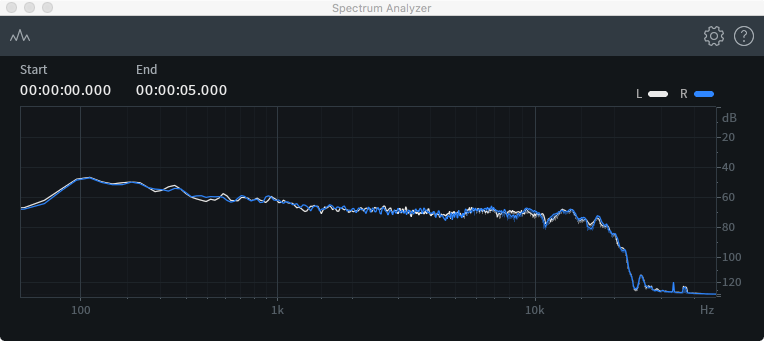
\includegraphics[width=.47\textwidth]{stereo-pairs-polar-patterns/PDF/AB.pdf}
% \caption{\textbf{AB}.}
% \label{AB}
% \end{center}
% \end{figure}
%-------------------------------------------------------------------------------
\subsubsection*{OSS}
% \vfill\null
% \begin{figure}[h]
% \begin{center}
% 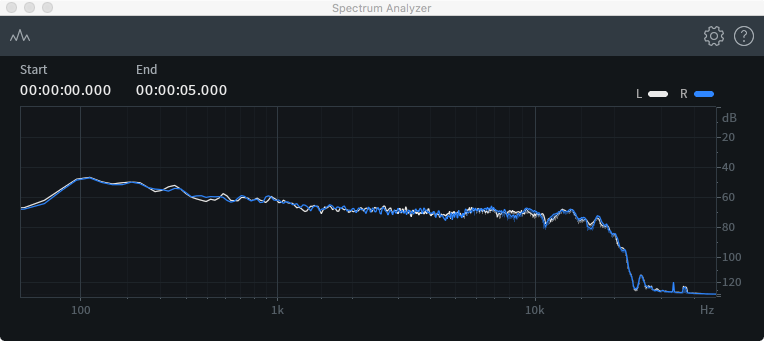
\includegraphics[width=.47\textwidth]{stereo-pairs-polar-patterns/PDF/AB.pdf}
% \caption{\textbf{AB}.}
% \label{AB}
% \end{center}
% \end{figure}
%-------------------------------------------------------------------------------
\subsubsection*{DECCA TREE}
% \vfill\null
% \begin{figure}[h]
% \begin{center}
% 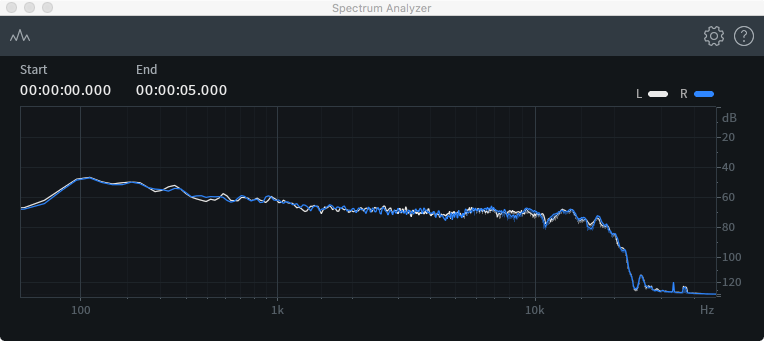
\includegraphics[width=.47\textwidth]{stereo-pairs-polar-patterns/PDF/AB.pdf}
% \caption{\textbf{AB}.}
% \label{AB}
% \end{center}
% \end{figure}
% \newpage % USE NEWPAGE TO FORCE COLUMNN INTERRUPTION
%-------------------------------------------------------------------------------
%-------------------------------------------------------------------------------
%\section*{UNNUMBERED SECTION}
%
% \begin{quote}
% La musica non e` solo composizione. \\
% Non è artigianato, non è un mestiere. \\
% La musica è pensiero. \cite{nono85}
% \end{quote}
%
% Some predictions of general relativity differ significantly from those of
% classical physics, especially concerning the passage of time, the geometry of
% space, the motion of bodies in free fall, and the propagation of light. Examples
% of such differences include gravitational time dilation, gravitational lensing,
% the gravitational redshift of light, and the gravitational time delay. The
% predictions of general relativity in relation to classical physics have been
% confirmed in all observations and experiments to date. Although general
% relativity is not the only relativistic theory of gravity, it is the simplest
% theory that is consistent with experimental data. However, unanswered questions
% remain, the most fundamental being how general relativity can be reconciled with
% the laws of quantum physics to produce a complete and self-consistent theory of
% quantum gravity.
%
% \begin{table}[htp]
% \begin{center}
% \begin{tabular}{ll}
% \textbf{Stages} & \textbf{Dur.} \\
% \hline
% \textbf{Omnidirectional Expositions} & 6 mo. \\
% Sound-shape analysis and visualizations & \\
% Sound-shape reproduction & \\
% Sound-shape database design & \\
% \hline
% \textbf{Micro-Rhythm of sound-shape} & 12 mo. \\
% Solo repertoire analysis & \\
% Sound-shape explosion in practising & \\
% From literature to shapes open-data & \\
% \hline
% \textbf{Rhythm of sound-shape interactions} & 12 mo. \\
% Multiple sources multiple shapes & \\
% Relationship and complexity perception & \\
% \hline
% \textbf{Sound-shape in musical composition} & 12 mo. \\
% AI: unleashed writing opportunities & \\
% AI: can you listen the time? & \\
% \hline
% \textbf{Final documentation} & 6 mo. \\
% \end{tabular}
% \label{timesheet}
% \caption{Thinking Tetrahedral Today stages}
% \end{center}
% \end{table}%
%
% Einstein's theory has important astrophysical implications. For example, it
% implies the existence of black holes regions of space in which space and time
% are distorted in such a way that nothing, not even light, can escape as an
% end state for massive stars. There is ample evidence that the intense radiation
% emitted by certain kinds of astronomical objects is due to black holes. For
% example, microquasars and active galactic nuclei result from the presence of
% stellar black holes and supermassive black holes, respectively. The bending of
% light by gravity can lead to the phenomenon of gravitational lensing, in which
% multiple images of the same distant astronomical object are visible in the sky.
% General relativity also predicts the existence of gravitational waves, which
% have since been observed directly by the physics collaboration LIGO. In addition,
% general relativity is the basis of current cosmological models of a consistently
% expanding universe. \cite{gerzon_70b}
%
% \begin{compactitem}
% \item Derivations of the Lorentz transformations
% \item Einstein–Hilbert action
% \item Tests of general relativity
% \item Two-body problem in general relativity
% \end{compactitem}
%
% \begin{figure}[t]
% \centering
% 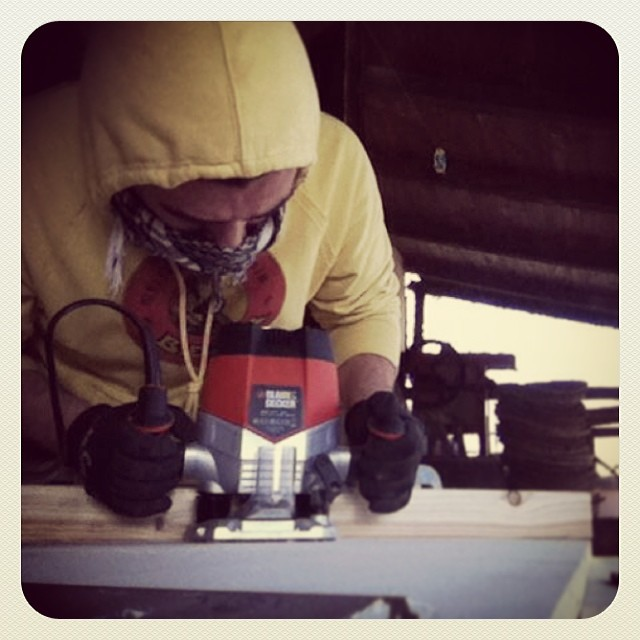
\includegraphics[width=.47\textwidth]{img/image2.jpg}
% \caption{Mind Mapping}
% \label{gs}
% \end{figure}
%
% \begin{equation}
% m(x,p,\theta) = (p*x) + ((1-p)*(x\cos\theta)
% \label{eq:mid}
% \end{equation}
%
% Some predictions of general relativity differ significantly from those of
% classical physics, especially concerning the passage of time, the geometry of
% space, the motion of bodies in free fall, and the propagation of light.

\vfill\null

\raggedright
\bibliographystyle{unsrt}
\bibliography{includes/bibliography.bib}

\end{document}

%%%%%%%%%%%%%%%%%%%%%%%%%%%%%%%%%%%%%%%%%%%%%%%%%%%%%%%%%%%%%%%%%%%%%%%%%%%%%%%%
% 2020 GIUSEPPE SILVI ARTICLE TEMPLATE BASED ON
%%%%%%%%%%%%%%%%%%%%%%%%%%%%%%%%%%%%%%%%%%%%%%%%%%%%%%%%%%%%%%%%%%%%%%%%%%%%%%%%
% Journal Article
% LaTeX Template
% Version 1.4 (15/5/16)
% This template has been downloaded from:
% http://www.LaTeXTemplates.com
% Original author:
% Frits Wenneker (http://www.howtotex.com) with extensive modifications by
% Vel (vel@LaTeXTemplates.com)
% License:
% CC BY-NC-SA 3.0 (http://creativecommons.org/licenses/by-nc-sa/3.0/)
%%%%%%%%%%%%%%%%%%%%%%%%%%%%%%%%%%%%%%%%%%%%%%%%%%%%%%%%%%%%%%%%%%%%%%%%%%%%%%%%
